\documentclass[times,t]{beamer}
\usepackage{amssymb}
\usepackage{amsmath}
\usepackage{amsfonts}
\usepackage{lmodern} 
\input{sym.tex}
\setbeamertemplate{navigation symbols}{}

\title{ECE 417/598: Line fitting using null space}
\author{Vikas Dhiman.  }
\date{March 11, 2022}
\begin{document}

\newcommand{\ubfu}{\underline{\bfu}}
\begin{frame}
  \titlepage
  \end{frame}
\begin{frame}
  \includegraphics[width=\linewidth]{media/lane-from-points.pdf}
  \begin{align*}
    \ubfu_1 &= [100, 98, 1]^\top\\
    \ubfu_2 &= [105, 95, 1]^\top\\
    \ubfu_3 &= [107, 90, 1]^\top\\
    \ubfu_4 &= [110, 85, 1]^\top
    \end{align*}
    Find  the line $\bfl$ such that it is the ``closest line'' passing through
    $\bfu_1, \dots, \bfu_4$.
\end{frame}

\begin{frame}
  \[
  U = \begin{bmatrix}\bfu_1^\top  \\
    \bfu_2^\top \\
    \bfu_3^\top \\
    \bfu_4^\top
  \end{bmatrix}
  \]
  We want to solve for $\bfl$ such that
  \[
    U \bfl = 0
  \]
\end{frame}

\begin{frame}{Singular Value  Decomposition (SVD)}
  \begin{align*}
    A  &=   U  \begin{bmatrix}\Sigma   &  0  \\   0  &  0 \end{bmatrix} V^\top
  \end{align*}
  \begin{align*}
    A^\top A &= V \Sigma^2  V^{-1}
  \end{align*}
  \begin{align*}
    A^\top A \bfv_i  &= \lambda_i \bfv_i & \lambda_i = \sigma_i^2\\
  \end{align*}
  \begin{align*}
    \bfu_i   &=  \frac{A\bfv_i}{\sigma_i}
    \end{align*}
    \begin{align*}
      U = \begin{bmatrix}
        \bfu_1 & \bfu_2 & \dots & \bfu_m
      \end{bmatrix}
    \end{align*}
\end{frame}

\begin{frame}
  \begin{align}
    A  &=   U  \begin{bmatrix}\Sigma   &  0  \\   0  &  0 \end{bmatrix} V^\top
  \end{align}
  If $A \in \bbR^{m \times n}$
  \begin{align}
    A = \begin{bmatrix}
      \bfu_1 & \bfu_2 & \dots & \bfu_m
    \end{bmatrix} \begin{bmatrix}
                 \sigma_1  & 0 & \dots & 0 & 0 & 0 & 0 \\
                 0 & \sigma_2 & \dots & 0 & 0 & 0 & 0\\
                 0 & 0 & \ddots & 0 & 0 & 0 & 0 \\
                 0 & 0 & 0 & \sigma_r & 0 & 0 & 0\\
                 0 & 0 & 0 & 0 & 0 & 0 & 0 \\
                 0 & 0 & 0 & 0 & 0 & 0 & 0
               \end{bmatrix}
                                     \begin{bmatrix}
                                       \bfv_1^\top \\
                                       \bfv_2^\top \\
                                       \vdots \\
                                       \bfv_n^\top
                                       \end{bmatrix}
  \end{align}
\end{frame}


\begin{frame}{Coding example}
  \begin{align*}
    \ubfu_1 &= [100, 98, 1]^\top\\
    \ubfu_2 &= [105, 95, 1]^\top\\
    \ubfu_3 &= [107, 90, 1]^\top\\
    \ubfu_4 &= [110, 85, 1]^\top
  \end{align*}
  Find  the line $\bfl$ such that it is the ``closest line'' passing through
  $\bfu_1, \dots, \bfu_4$.
  \url{https://github.com/wecacuee/ECE417-Mobile-Robots/tree/master/docs/slides/03-09-svd-null-space}
\end{frame}

\begin{frame}
  \[
    A = \begin{bmatrix}\bfu_1^\top  \\
      \bfu_2^\top \\
      \bfu_3^\top \\
      \bfu_4^\top
    \end{bmatrix}
  \]
  We want to solve for $\bfl$ such that
  \[
    U \bfl = 0
  \]
\end{frame}


\begin{frame}{Homography}
  \includegraphics[width=\linewidth]{media/homography-maps-a-line-to-a-line.png}
\end{frame}
\begin{frame}{Examples  of  Homography}
  \includegraphics[width=\linewidth]{media/examples-of-homography.png}
\end{frame}

\begin{frame}
  \includegraphics[width=0.60\linewidth]{media/audi top view camera.jpg}
\end{frame}

\begin{frame}{Computing Homography}
  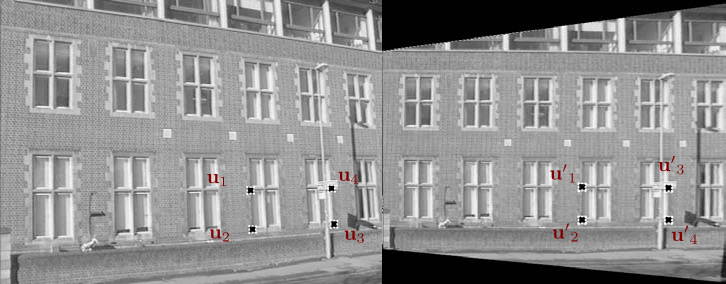
\includegraphics[width=0.45\linewidth]{media/removing-perspective-distortion.png}
  \includegraphics[width=0.45\linewidth]{media/removing-perspective-distortion-b.png}
\end{frame}


\begin{frame}{Computing Homography}
  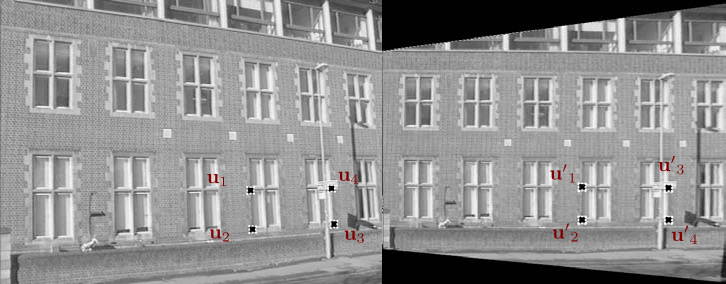
\includegraphics[width=0.45\linewidth]{media/removing-perspective-distortion.png}
  \includegraphics[width=0.45\linewidth]{media/removing-perspective-distortion-b.png}
\end{frame}

\begin{frame}{Solving for Homography derivation}
\end{frame}

\begin{frame}{Direct Linear Transformation   (DLT) algorithm}
  \includegraphics[width=\linewidth]{media/DLT-algorithm.png}
\end{frame}

\begin{frame}{2D homography}
  Given a set of points $\bfx_i \in \bbP^2$ and a corresponding set of
  points $\bfx'_i \in \bbP^2$, compute the projective transformation that takes each
  $\bfx_i$ to $\bfx'_i$ . In a practical situation, the points $\bfx_i$ and   $\bfx'_i$  are points in two images
  (or the same image), each image being considered as a projective plane  $\bbP^2$.
\end{frame}

\begin{frame}{3D  to  2D camera projection matrix estimation}
  Given a set of points $\bfX_i$ in 3D space, and a set
  of corresponding points $\bfx_i$ in an image, find the 3D to 2D projective
  $\bfP$ mapping
  that maps $\bfX_i$ to $\bfx_i  =  \bfP\bfX_i$.
\end{frame}

\end{document}